\documentclass[lettersize,journal,onecolumn]{IEEEtran}
\usepackage{amsmath,amsfonts}
\usepackage{algorithmic}
\usepackage{array}
\usepackage[caption=false,font=normalsize,labelfont=sf,textfont=sf]{subfig}
\usepackage{textcomp}
\usepackage{stfloats}
\usepackage{url}
\usepackage{verbatim}
\usepackage{graphicx}
\hyphenation{op-tical net-works semi-conduc-tor IEEE-Xplore}
\def\BibTeX{{\rm B\kern-.05em{\sc i\kern-.025em b}\kern-.08em
    T\kern-.1667em\lower.7ex\hbox{E}\kern-.125emX}}
\usepackage{balance}
\begin{document}

%\title{How to Use the IEEEtran \LaTeX \ Templates}
\title{Dispositivo medico-estetico ViBra 2.0}
\author{Relatore: Roberto ROBORTELLA - roberto.robortella@supsi.ch - Ufficio: 2.01 BB \newline
Co-Relatore: Christian TAVILLA - agatinochristian.tavilla@supsi.ch - Ufficio: 3.07 BB}

\markboth{Progetto di Diploma, Maggio~2024}%
{How to Use the IEEEtran \LaTeX \ Templates}

\maketitle

%\begin{abstract}
%This document describes the most common article elements and how to use the IEEEtran class with \LaTeX \ to produce files that are suitable for submission to the Institute of Electrical and Electronics Engineers (IEEE).  IEEEtran can produce conference, journal and technical note (correspondence) papers with a suitable choice of class options.
%\end{abstract}

%\begin{IEEEkeywords}
%Class, IEEEtran, \LaTeX, paper, style, template, typesetting.
%\end{IEEEkeywords}
\section{Introduzione}
\IEEEPARstart{V}{iBra 2.0} nasce come studio alternativo ad un attuale prodotto, commercializzato da un nostro partner, attualmente sul mercato.
Il prodotto attuale (ViBra 1.0) produce delle variazioni di pressione, applicate con specifiche cupole, sui tessuti del paziente che tramite le conseguenti vibrazioni stimola i tessuti sottostanti tonificando e migliorandone la circolazione.
Il dispositivo possiede 14 uscite sincrone, attivate da una soffiante a canali laterali, che convoglia il flusso in un frazionatore che alterna i flussi entata-uscita della soffiante ad ogni uscita.
\section{Nuovo design: Intenti e \\ Limitazioni}
\noindent Affinché si possa migliorare il prodotto attuale (1.0), elenchiamo qui di seguito alcuni dei limiti attuali che motivano lo studo di un nouvo approccio:
\begin{list}{}{}
\item{- Numero di canali: (14) Fisso;}
\item{- Forma d'onda: fissa (pseudo sinusoidale);}
\item{- Velocità di pulsazone: Unica per tutti i canali (30-500Hz);}
\item{- Notevole ingombro dovuto alla soffiante e al frazionatore;}
\item{- Notevole costo per soffiante e frazionatore.}
\end{list}
Nel nuovo prodotto si vorrebbe ottenere:
\begin{list}{}{}
\item{- Numero di canali: (14) Selezionabili separatamente;}
\item{- Forma d'onda: Selezionabile;}
\item{- Visualizzazione della pressione applicata al paziente;}
\item{- Velocità di pulsazone: Separata per tutti i canali (30-500Hz);}
\item{- Riduzione degli ingombri generali rispetto al design 1.0;}
\item{- Riduzione dei costi realizzativi.}
\end{list}
\section{Progetto di studio}
\noindent Considerate le limitazioni tecniche del macchinario attuale e l'impossibilità di utilizzare trattamenti a pressioni e frequenze diverse per ogni attuatore, si vorrebbe realizzare, tramite attuatore elettroacustico, un sistema a canali indipendenti e parametrizzabili singolarmente. Per questo studio ci limiteremo ad un singolo canale.
\noindent Il range di pressioni di lavoro dovranno essere compresi tra +/-250 mBar per frequenze di stimolazione comprese tra 30Hz e 500Hz.
\subsection{Compiti}
\noindent I seguenti compiti saranno da portare a termine:
\begin{enumerate}{}{}
\item Definire le specifiche di sistema in accordo con il relatore;
\item Definire l'architettura per l'implementazione;
\item Definire l'hardware necessario all'implementazione;
\item Valutare l'elettronica necessaria all'attuazione, alla misura e al controllo delle variabili di funzionamento;
\item Proporre una configurazione hardware (meccanica ed elettronica) per realizzare il dispositivo mono/duo-canale;
\item Realizzare meccanica, elettronica e firmware per un banco dimostrativo funzionale.
\end{enumerate}
\subsection{Schema funzionale}
\noindent La realizzazione dovrà indicativamente rappresentare lo schema seguente, che si compone di:
\begin{enumerate}{}{}
\item \textbf{Alimentazione (Supply) :} produce le alimentazioni neccessarie al funzionamento del dispositivo a partire da una sorgente 24VDC (ev. da ridefinire secondo le specifiche del driver, ma non oltre 48VDC).
\item \textbf{Driver :} fornisce i segnali di comando in potenza all'attuatore elettroacustico. Idealmente in classe D.
\item \textbf{Display Touch :} fornisce una interfaccia utente per l'impostazione dei parametri di funzionamento e monitora le variabili di sistema e i segnali.
\item \textbf{Sensore di posizione :} misura lo spostamento della membrana.
\item \textbf{Sensori di pressione :} misurano la pressione applicata alle cupole di applicazione al paziente.
\item \textbf{Controllo :} implementa un sistema di controllo sui segnali di attivazione dell'attuatore in funzione dei sensori letti (pressione e posizione della membrana) permettendo una stimolazione controllata e la messa in sicurezza dell'attuatore nei suoi possibili regimi di funzionamento. Idealmente in forma PID per il controllo di pressione, con intervento in modalità soglia per la limitazione dello spostamento della membrana (soprattutto in modalità bi-canale). 
\item \textbf{Microcontrollore (uC) :} Permette l'interazione con l'interfaccia utente (Display Touch), genera i segnali di stimolo, legge i sensori e gestisce il sistema nel suoi intero. Eventualmente implementa una forma di controllo digitale della parte PID e di limitazione.
\item \textbf{Attuatore :} produce l'onda di pressione elettroacustica. Idealmente di tipo sub-woofer con alto $x_{max}$.
\end{enumerate}

\begin{figure}[!t]
\centering
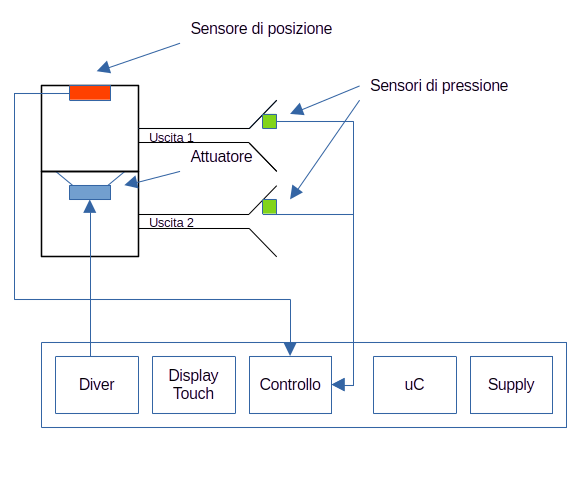
\includegraphics[width=4in]{figA}
\caption{Schema di principio}
\label{figA}
\end{figure}

\subsection{Obiettivi}
\noindent I seguenti obbiettivi di progetto/tesi dovranno essere raggiunti:
\begin{enumerate}{}{}
\item{Definire le specifiche iniziali;}
\item{Studiare ed implementare tramite stampa 3D la struttura meccanica del blocco di attuazione sulla base dell'attuatore selezionato;}
\item{Studiare, simulare, dimensionare ed implementare una scheda elettronica che racchiuda: Display Touch, microcontrollore, controllore, driver, sensori, alimentazione;}
\item{Realizzare un banco prova/dimostratore;}
\item{Definire delle specifiche finali sotto forma di datasheet;}
\item{Redazione della documentazione relativa al progetto: Poster, Presentazione, Rapporto (\LaTeX).}
\end{enumerate}
\subsection{Tecnologie}
\noindent Tramite questo progetto, i seguenti ambiti e tecnologie saranno affrontati:
\begin{enumerate}{}{}
\item Elettronica analogica e/o mixed signal (Driver/sensorica/PID);
\item Conversione energetica DC/DC;
\item Amplificazione in gamma audio con stadio in classe-D;
\item Programmazione Microcontrollore STM32 (idealmente STM32F469i-DISCO);
\item Disegno CAD e stampa 3D (AutoCad Inventor o FreeCad o altro);
\item Dimensionamento e simulazione elettroacustica con parametri Thiele \& Small (WinISD o simili);
\item Disegno CAD di schematico e PCB (Altium o Eagle o KiCad);
\item Stesura documentazione il \LaTeX (Texmaker o LED o OverLeaf).
\end{enumerate}
\end{document}


